%% LyX 2.0.5.1 created this file.  For more info, see http://www.lyx.org/.
%% Do not edit unless you really know what you are doing.
\documentclass[usenatbib]{article}
\usepackage[latin9]{inputenc}
\usepackage[a4paper]{geometry}
\geometry{verbose}
\usepackage{graphicx}

\makeatletter

%%%%%%%%%%%%%%%%%%%%%%%%%%%%%% LyX specific LaTeX commands.
%% A simple dot to overcome graphicx limitations
\newcommand{\lyxdot}{.}


%%%%%%%%%%%%%%%%%%%%%%%%%%%%%% Textclass specific LaTeX commands.
\usepackage{jcappub}

%%%%%%%%%%%%%%%%%%%%%%%%%%%%%% User specified LaTeX commands.






%%%%%%%%%%%%%%%%%%%%%%%%%%%%%% LyX specific LaTeX commands.
%% A simple dot to overcome graphicx limitations
%Make my life significantly easier
\global\long\def\bd{{\bm{\delta}}}

\makeatother

\begin{document}

\title{The Maximum Circular Velocity Dependence of Halo Clustering}

\maketitle

\section{Introduction}

XXX


\section{The Simulation}

We use cosmological N-body simulations called the Bolshoi simulation
and the MultiDark simulation, described in XXX and XXX respectively,
to investigate the maximum circular velocity dependence of halo clustering.
The Bolshoi simulation uses $2048^{3}$ particles with a volume of
$(250$$h^{-1}{\rm Mpc})^{3}$, while the MultiDark simulation uses
the same number of particles as the Bolshoi simulation but with a
volume of ($1h^{-1}{\rm Gpc})^{3}$. Both simulations assumes a flat
$\Lambda{\rm CDM}$ model with density parameters $\Omega_{m}=0.27$,
$\Omega_{\Lambda}=0.73$, $\Omega_{b}=0.0469$, and $\sigma_{8}=0.82$,
$n=0.95$, the Hubble parameter $h=0.70$. The details of the simulations
are described in XXX. For halo identification, we use the ROCKSTAR
halo finder (XXX) where the halo masses and maximum circular velocities
are computed from bound particles.


\section{The Maximum Circular Velocity Dependence of Halo Clustering}

In this section, we investigate the maximum circular velocity dependence
of halo clustering. As shown in Fig. XXX, the maximum circular velocity
and halo mass has tight correlation, and yet the scatter between the
maximum circular velocity and halo mass becomes larger with decreasing
halo masses. In fact, we can compute an expected maximum circular
velocity from halo mass such as

\begin{equation}
V_{max}=0.465M_{vir}^{1/3}\sqrt{G(\frac{4}{3}\pi\Delta_{h}\rho_{crit}\Omega_{m})^{1/3}\frac{c}{{\rm ln(1+c)-c/(1+c)}}},\label{eq:vmax-mvir}
\end{equation}
where $V_{max}$ is the maximum circular velocity and $M_{vir}$ is
the halo mass, $G$ is the gravitational constant, $\Delta_{h}$ is
XXX, and $c$ is the concentration parameter. To obtain Eq. \ref{eq:vmax-mvir},
we use the concentration of 
\begin{equation}
{\rm log}_{10}c=-0.097{\rm log_{10}M_{vir}}+2.148.
\end{equation}
(Ask Frank how he obtain this concentration value and why this is
a reasonable value + do I need more explanation for Eq. 1? How should
I call this relationship?)

\begin{figure}
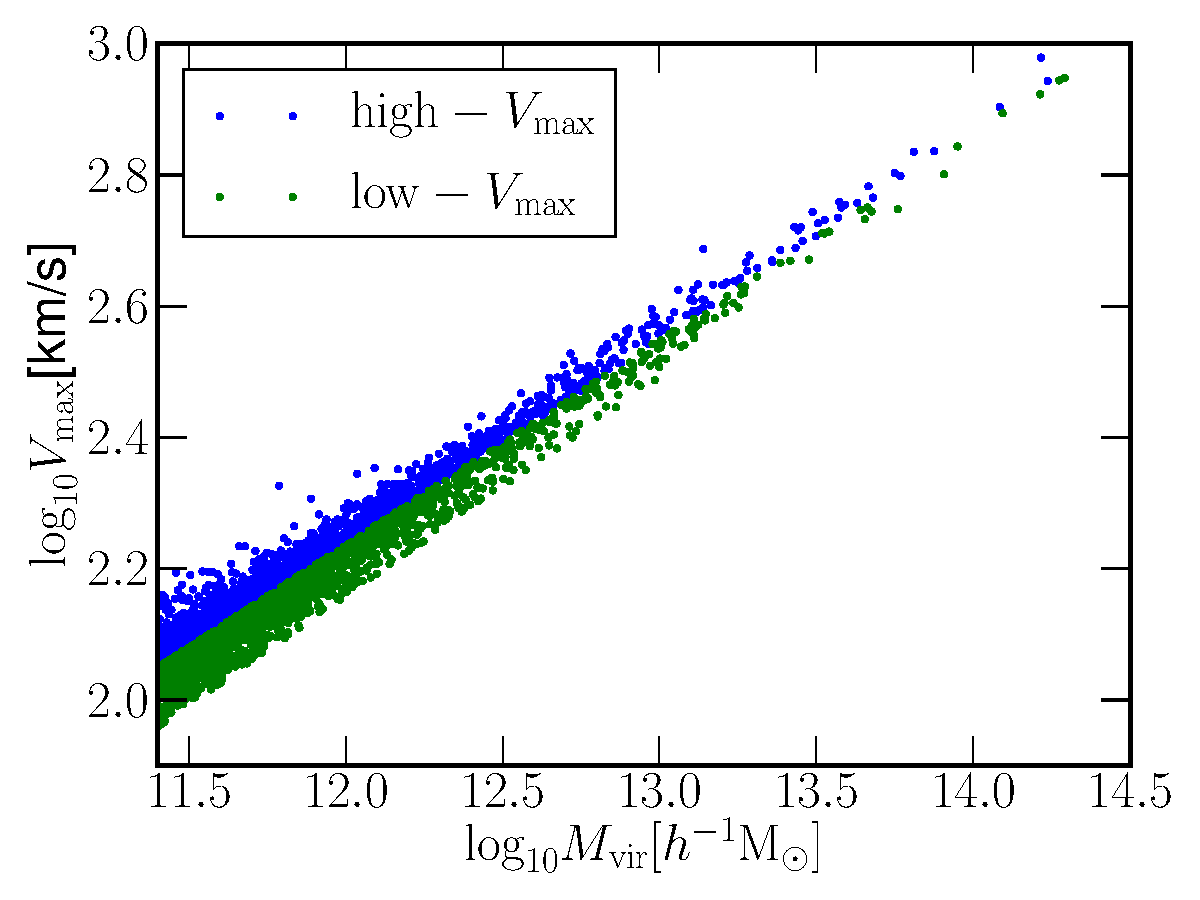
\includegraphics[width=0.5\columnwidth]{\lyxdot \lyxdot /Downloads/logVmax_logMvir_Dh360}

\caption{\label{fig:vmax-mvir}Distribution of halo mass and the maximum circular
velocity at $z=0.0$ from the MultiDark simulation. The red solid
line represents the maximum circular velocity computed from the halo
mass using Eq. XXX. The red and green dashed lines are $1\sigma$
and $2\sigma$ away in the log-normal distribution of concentration
at a fixed halo mass.}
\end{figure}


We use the expected maximum circular velocity from Eq. \ref{eq:vmax-mvir}
to split each mass bin into two subsamples, ``upper'' and ``lower''
subsamples where halos have greater (or lower) maximum circular velocity
than the expected value. We compute halo-matter cross correlation
functions for each subsample and obtain a linear bias such as 
\begin{equation}
b_{lin}=<\xi_{hm}(r)/\xi_{mm}(r)>,
\end{equation}
where $\xi_{hm}$ and $\xi_{mm}$ are halo-matter and matter-matter
correlation functions and we take the average of the ratio on $r$
from $10h^{-1}{\rm Mpc}$to $20h^{-1}{\rm Mpc}$. Fig. \ref{fig:linear-bias}
shows a linear bias as a function of halo mass for ``upper'' and
``lower'' maximum circular velocity halos. The halos which have
different maximum circular velocity clearly cluster differently. In
Fig. \ref{fig:linear-bias-ratio}, we take the ratio of those two
subsamples to show more directly how the effect of the maximum circular
velocity becomes larger on lower halo masses.

\begin{figure}
\includegraphics[width=0.5\columnwidth]{\lyxdot \lyxdot /Downloads/linearBias_wang2_Bolshoi4}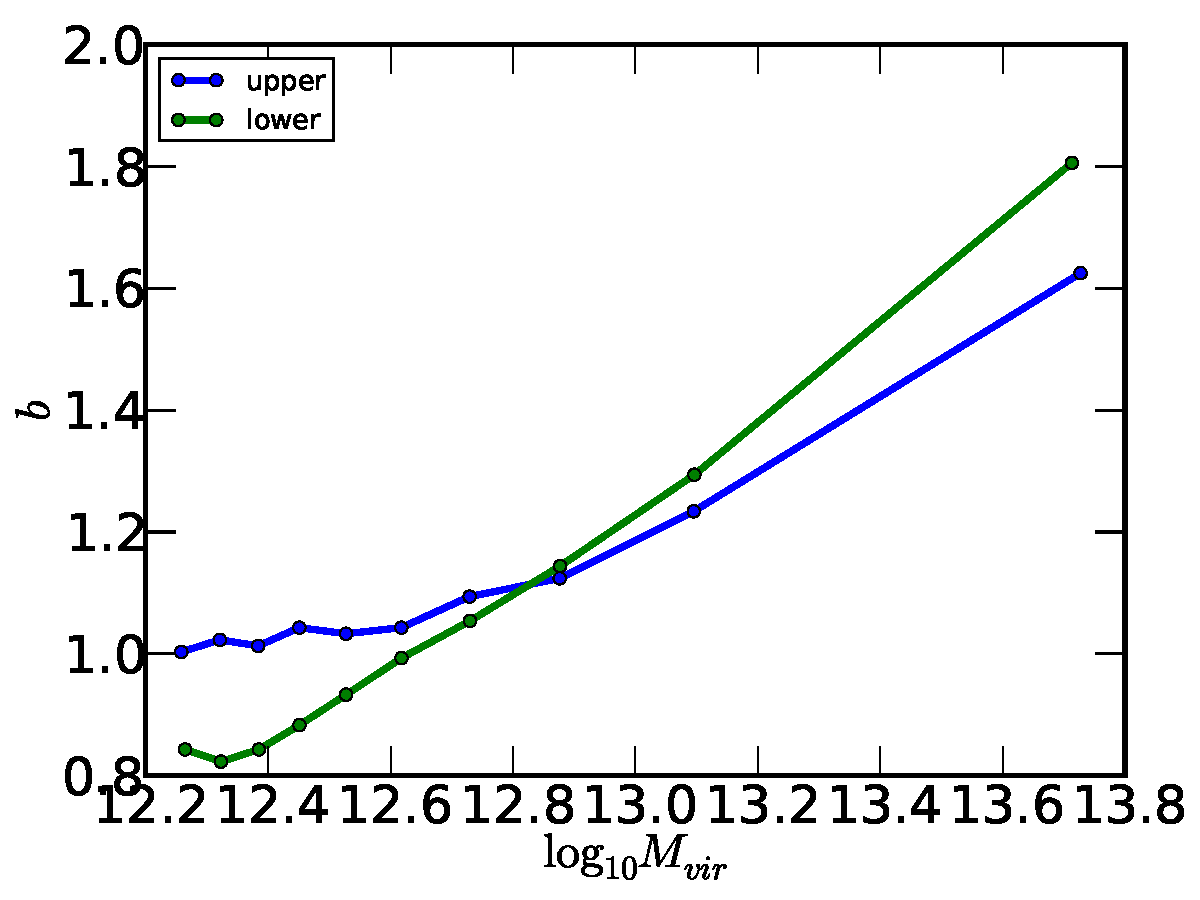
\includegraphics[width=0.5\columnwidth]{\lyxdot \lyxdot /Downloads/linearBias_wang2_MultiDark}

\caption{\label{fig:linear-bias}Linear bias at $z=0.0$ as a function of halo
mass from the Bolshoi simulation (left) and the MultiDark simulation
(right). The blue solid line represents a linear bias for halos whose
maximum circular velocities are greater than the expected value obtained
from Eq. \ref{eq:vmax-mvir} (labeled as ``upper''), while the green
solid line corresponds to halos whose maximum circular velocities
are smaller than the expected (labeled as ``lower''). Both plots
indicate the maximum circular velocity dependence of clustering as
a function of halo mass. The relative bias of upper versus lower maximum
circular velocity halos increases with decreasing halo masses.}
\end{figure}


\begin{figure}
\includegraphics[width=0.5\columnwidth]{\lyxdot \lyxdot /Downloads/linearBiasRatio_wang2_Bolshoi4}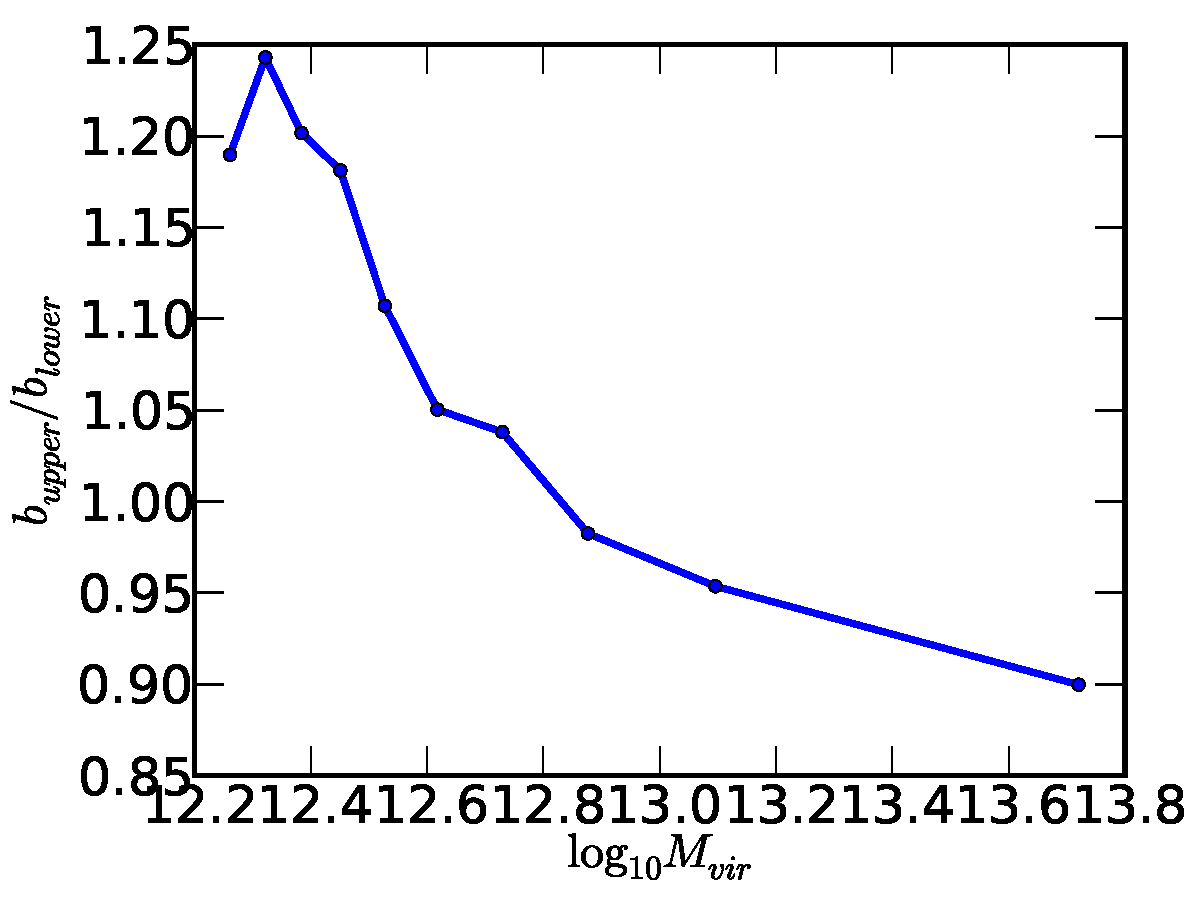
\includegraphics[width=0.5\columnwidth]{\lyxdot \lyxdot /Downloads/linearBiasRatio_wang2_MultiDark}

\caption{\label{fig:linear-bias-ratio}Ratio of linear biases between ``upper''
and ``lower'' maximum circular velocity halos at $z=0.0$ from the
Bolshoi simulation (left) and the MultiDark simulation (right). The
maximum circular velocity dependence becomes stronger as halo mass
decreases.}


\end{figure}


We also investigate how the scale-dependence of halo bias can differ
for halos which have different maximum circular velocities. Fig. \ref{fig:small-scale}
shows the ratio of halo-matter cross correlation functions between
``upper'' and ``lower'' subsamples on small scales. For lower
mass halos, the effect on the scale-dependence of halo bias becomes
larger.

\begin{figure}
\includegraphics[width=0.5\columnwidth]{\lyxdot \lyxdot /Downloads/Bolshoi4_smallScale_wang2}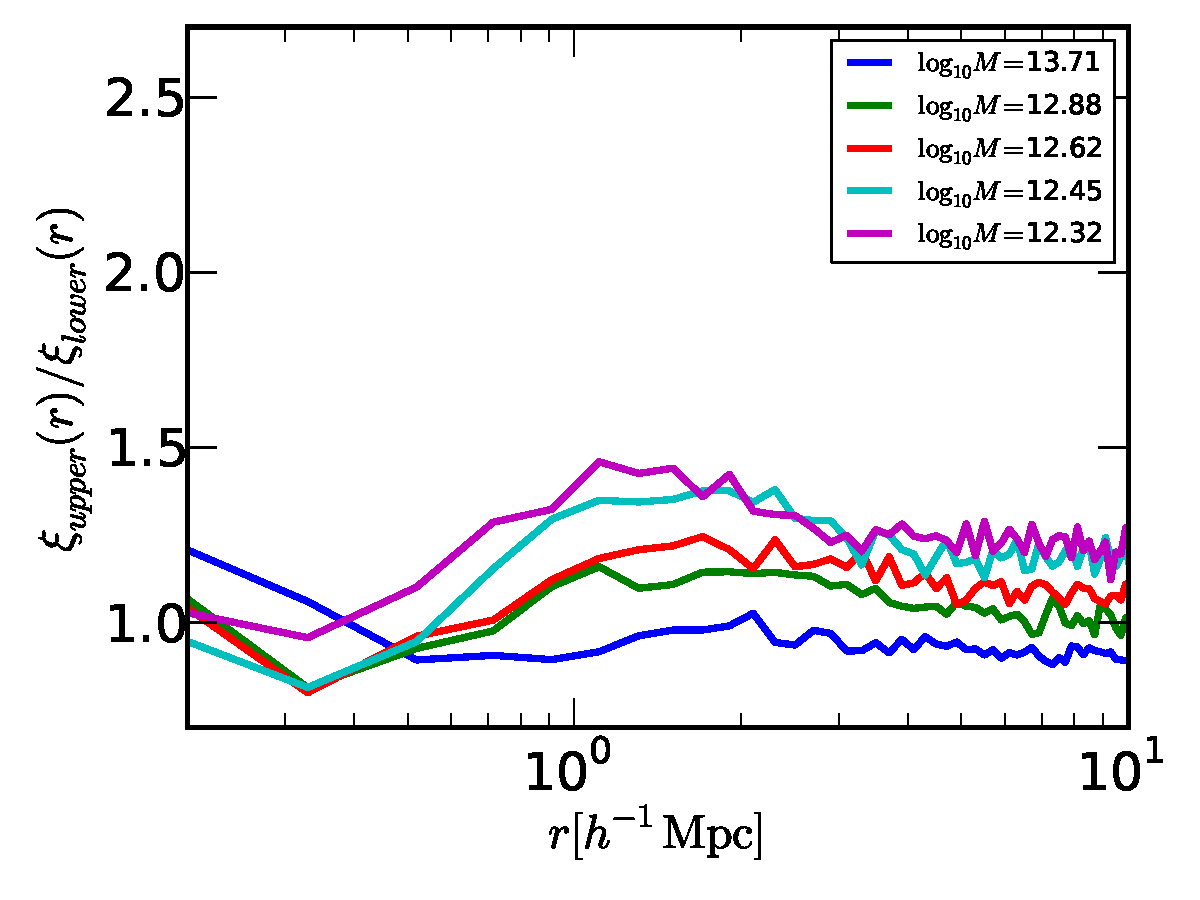
\includegraphics[width=0.5\columnwidth]{\lyxdot \lyxdot /Downloads/MultiDark_smallScale_wang2}

\caption{\label{fig:small-scale}Ratio of halo-matter cross correlation functions
for ``upper'' and ``lower'' maximum circular velocity halos on
small scales from the Bolshoi simulation (left) and the MultiDark
simulation (right) at $z=0.0$. Each line corresponds to different
halo mass bin as shown in the plots. The plots show that halos which
have different maximum circular velocity have different scale dependence
of halo bias.}


\end{figure}



\section{Discussion}
\end{document}
